\documentclass[accentcolor=tud1b,colorbacktitle,inverttitle,landscape,presentation,t]{tudbeamer}
\usepackage[utf8]{inputenc}
\usepackage[german]{babel}
\usepackage{verbatim, hyperref,multimedia}
\usepackage{graphicx, psfrag}			%to insert graphics
\usepackage{setspace}
\usepackage[active]{srcltx}
\usepackage{color}
\usepackage{subfigure}
\usepackage{listings}
\usepackage{pstricks}
\usepackage{amssymb}

\useinnertheme{default}
\usecolortheme{orchid}
\setbeamercovered{transparent}


\newcommand{\keyword}[1]{\textcolor{tudaccent}{\textbf{#1}}}
\newcommand{\myframetitle}[2]{\frametitle{#1 \\[.2cm] \small #2}}
\newcommand{\fatitem}[1]{\item \textbf{#1}}
\newcommand{\tab}{\hspace*{0.5cm}}


\setcounter{tocdepth}{1} 

\hypersetup{
pdftitle={WebMining Exercise }, pdfauthor={F. Englert}
}


\begin{document}

\title[MGA]{\large 1. Exercise}

\author{Frank Englert, Jens Haase}
\institute{KE, TU Darmstadt}

\logo{
\includegraphics{keicon.png}}

\date{April 2011}

\begin{titleframe}
\begin{center}
\color{tudtextaccent} \large The first exercise\\[.5cm]
%\includegraphics[width=0.4\textwidth]{Graphics/spg_logo_final.eps} \\
\normalcolor \normalsize Knowlege Engineering \\
Fachbereich Informatik \\
Technische Universität Darmstadt\\[.5cm]

\textbf{Exercise Presentation:}\\
Frank Englert\\
Jens Haase
\end{center}

\end{titleframe} 

\begin{frame}[c]
	\myframetitle{1. Exercise}{Overview}
\begin{enumerate}
  \item Webmining Application Example
  \item Word Count
  \item Probability of Word occurences
  \item Probability of Silbing occurences
  \item Language Detection Plugin for Firefox
\end{enumerate}
\end{frame}

\begin{frame}[c]
	\myframetitle{Task 1 - Language detection}{Language Detection via letter
	distribution}
\begin{itemize}
  \item The Firefox Plugin uses two detection modes
  \begin{itemize}
    \item Via letter frequency analysis
    \item Via syllable frequency analysis
  \end{itemize}
  \item The language detection algorithm is the same for both cases
  \item Advantages of using two detection modes:
  \begin{itemize}
    \item Double check the language detection results
    \item Collect information which mode works better
  \end{itemize}
  \item The Source of the frequency tables is http://bit.ly/jZHf0H
\end{itemize}
\end{frame}

\begin{frame}[c]
\myframetitle{Task 1 - Language detection}{Algorithm details}
\begin{itemize}
  \fatitem{The algorithms works with the following steps}
  \item A chunk is either a letter or a syllable
  \item dict contains the most important chunks of a language sorted by rank
\begin{enumerate}
  \item Take the text an split it to chunks(letters or syllables)
  \item Remove all chunks which are not in the dict
  \item Count the chunks and sort them by the count value. The result of this
  step is further called rankedChunks
  \item The weighted difference between the dictionary and the rankedChunks is
  \begin{itemize}
  \item $ \sum _{i=0}^{len(dic)} \frac{| i - rankedChunks.indexOf(dict[i]) |
  }{log _2 (i+2)}
  $
  \item If dict and rankedChunks are equals the weighted difference is 0
\end{itemize}
\end{enumerate}
\item repeat the steps 1-4 for all available languages. Take the language with
the lowest rank.
\end{itemize}
\end{frame}

\begin{frame}[c]
	\myframetitle{Task 1 - Language detection}{Letter frequency revisited}
\begin{figure}[htp]
\begin{center}
  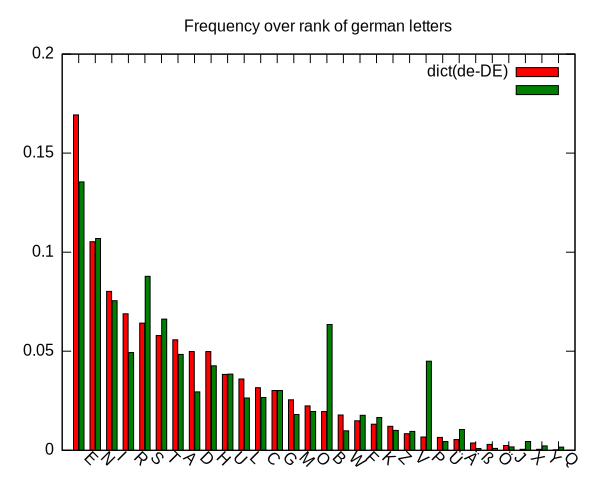
\includegraphics[width=1\textheight]{graphics/letters_de}
  \caption[fig:letters_de]{The frequency of german letters used
  for the Firefox plugin}
  \label{figureLabel}
\end{center}
\end{figure}

\end{frame}

\begin{frame}[c]
	\myframetitle{Task 1 - Language detection}{Syllable frequency revisited}

\begin{figure}[htp]
\begin{center}
  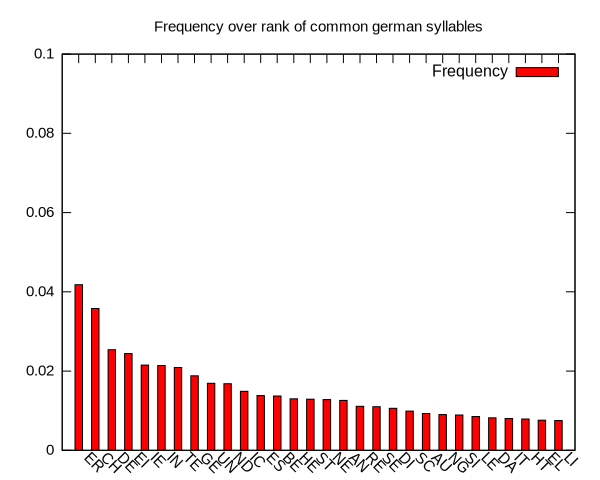
\includegraphics[width=1\textheight]{graphics/syllables_de}
  \caption[fig:letters_de]{The frequency of common german syllables used for the Firefox plugin}
  \label{figureLabel}
\end{center}
\end{figure}

\end{frame}


\begin{frame}[c]
	\myframetitle{Task 1 - Language detection}{Results of the language challenge}

\begin{table}
\begin{tabular}{|l|l|l|}
\hline
\textbf{Rank} &\textbf{letter lang}&\textbf{syllable lang}\\
\hline
1 &englisch&-\\
2 &englisch&-\\
3&deutsch&-\\
4&französisch&-\\
5&deutsch&-\\
6&deutsch&deutsch\\
7&französisch&französisch\\
8&französisch&französisch\\
9&englisch&englisch\\
10&deutsch&deutsch\\
\hline
\end{tabular}
\caption{Detection results of the firefox plugin}
\label{tablelabel}
\end{table}

\end{frame}

\begin{frame}[c]
	\myframetitle{Task 1 - Language detection}{Further improvement}
	
	\begin{itemize}
	\fatitem{Easy:}
	\begin{itemize}
		\item Add more languages
	\end{itemize}
	
	  \fatitem{A lot of work:}
	  \begin{itemize}
  	    \item The Plugin checks already p, div and span tags. It would be better
  	  to check the text content of all tags.
  	    \item Try to estimate the best detection result if the syllable and the
  	letter mode returns different results
      \end{itemize}
      \fatitem{Most Interesting:}
      \begin{itemize}
  		\item Improve the weighting algorithm to reduce the amount of needed text
  		\item Implement a learning mode to train new languages

	\end{itemize}
	\end{itemize}
\end{frame}
\begin{frame}[c]
	\myframetitle{Task 2 }{}
\begin{itemize}
  \item ...
\end{itemize}
\end{frame}


\begin{frame}[c]
	\myframetitle{Probability of Word occurences}{Zipf's law (linear scale)}
	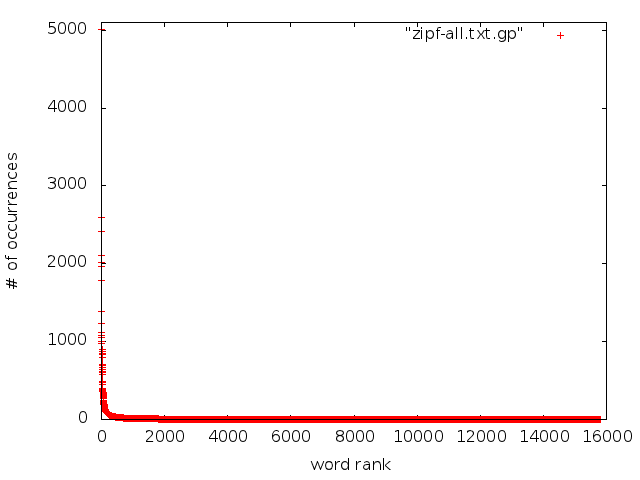
\includegraphics[scale=0.4]{../task02-04/src/main/resources/results/task3/zipf-lin.png}
\end{frame}

\begin{frame}[c]
	\myframetitle{Probability of Word occurences}{Zipf's law (log scale)}
	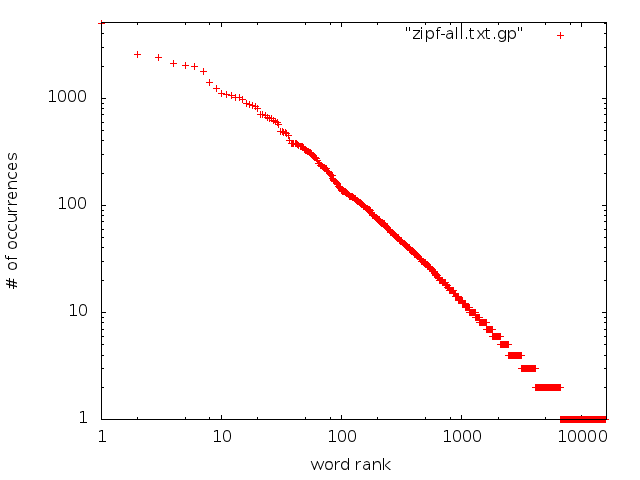
\includegraphics[scale=0.4]{../task02-04/src/main/resources/results/task3/zipf-log.png} 
\end{frame}	

\begin{frame}[c]
	\myframetitle{Probability of Word occurences}{Probability of Frequency (linear scale)}
	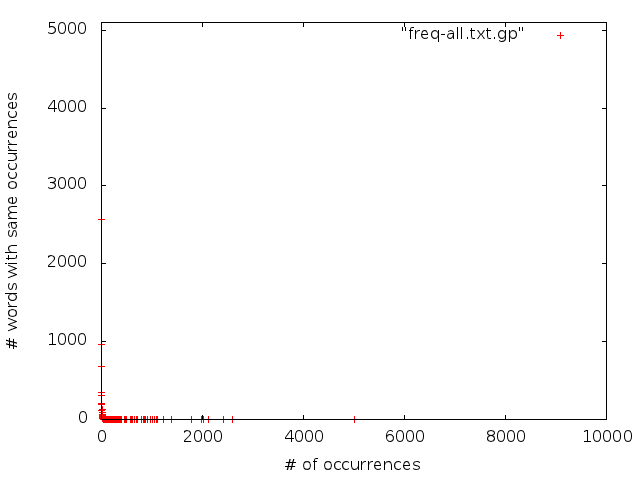
\includegraphics[scale=0.4]{../task02-04/src/main/resources/results/task3/freq-lin.png}
\end{frame}

\begin{frame}[c]
	\myframetitle{Probability of Word occurences}{Probability of Frequency (log scale)}
	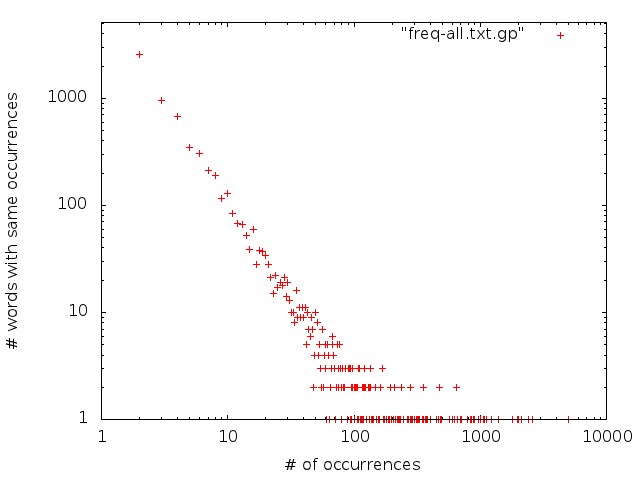
\includegraphics[scale=0.4]{../task02-04/src/main/resources/results/task3/freq-log.png} 
\end{frame}	
\begin{frame}[c]
	\myframetitle{Task 4}{Evaluation von GZip}
\begin{itemize}
  \fatitem{Klassifikationsmatrix für GZip(Kompressionsstufe 1)}
 \begin{table}[htbp]
\begin{tabular}{|l|r|r|r|r|r|r|r|}
\hline
train$\downarrow$ test$\rightarrow$& \multicolumn{1}{l|}{project} &
\multicolumn{1}{l|}{course} & \multicolumn{1}{l|}{other} & \multicolumn{1}{l|}{student} &
\multicolumn{1}{l|}{faculty} & \multicolumn{1}{l|}{dpt.} &
\multicolumn{1}{l|}{staff} \\ \hline project & 6 & 0 & 5 & 8 & 2 & 27 & 203 \\ \hline course & 3 & 29 & 7 & 22 & 14 & 57 & 332 \\ \hline other & 45 & 71 & 106 & 85 & 67 & 256 & 1250 \\ \hline
student & 5 & 4 & 39 & 73 & 47 & 87 & 565 \\ \hline
faculty & 1 & 2 & 8 & 21 & 48 & 38 & 443 \\ \hline
dpt. & 0 & 0 & 1 & 3 & 1 & 38 & 46 \\ \hline
staff & 0 & 0 & 1 & 2 & 3 & 8 & 53 \\ \hline
\end{tabular}
\caption{Resultate für GZip Kompressionsstufe 1}
\label{tbl:GzipL1}
\end{table}
 
\end{itemize}
\end{frame}

\begin{frame}[c]
\myframetitle{Task4}{Evaluation von GZip}
\begin{itemize}
  \fatitem{Klassifikationsmatrix für GZip(Kompressionsstufe 2)}
  \begin{table}[htbp]
\caption{Resultate für GZip Kompressionsstufe 2}
\begin{tabular}{|l|r|r|r|r|r|r|r|}
\hline
train$\downarrow$ test$\rightarrow$& \multicolumn{1}{l|}{project} & \multicolumn{1}{l|}{course} &
\multicolumn{1}{l|}{other} & \multicolumn{1}{l|}{student} &
\multicolumn{1}{l|}{faculty} & \multicolumn{1}{l|}{dept.} &
\multicolumn{1}{l|}{staff} \\ \hline project & 55 & 4 & 0 & 38 & 27 & 0 & 127 \\ \hline course & 105 & 6 & 0 & 73 & 44 & 0 & 236 \\ \hline other & 356 & 64 & 0 & 308 & 180 & 0 & 972 \\ \hline
student & 174 & 25 & 0 & 121 & 78 & 0 & 422 \\ \hline
faculty & 115 & 15 & 0 & 77 & 65 & 0 & 289 \\ \hline
dept. & 13 & 0 & 0 & 18 & 13 & 0 & 45 \\ \hline
staff & 18 & 2 & 0 & 10 & 5 & 0 & 32 \\ \hline
\end{tabular}
\label{tbl:GzipL2}
\end{table}
  
   
\end{itemize}
\end{frame}

\begin{frame}[c]
\myframetitle{Task4}{Evaluation von GZip}
\begin{itemize}
  \fatitem{Klassifikationsmatrix für GZip(Kompressionsstufe 6)}
  \begin{table}[htbp]
\caption{Resultate für GZip Kompressionsstufe 6}
\begin{tabular}{|l|r|r|r|r|r|r|r|}
\hline
train$\downarrow$ test$\rightarrow$& \multicolumn{1}{l|}{project} & \multicolumn{1}{l|}{course} &
\multicolumn{1}{l|}{other} & \multicolumn{1}{l|}{student} &
\multicolumn{1}{l|}{faculty} & \multicolumn{1}{l|}{dept.} &
\multicolumn{1}{l|}{staff} \\ \hline project & 25 & 0 & 19 & 8 & 6 & 3 & 190 \\ \hline course & 16 & 88 & 19 & 27 & 12 & 6 & 296 \\ \hline other & 136 & 109 & 125 & 112 & 53 & 60 & 1285 \\ \hline
student & 17 & 1 & 88 & 106 & 38 & 4 & 566 \\ \hline
faculty & 2 & 2 & 13 & 19 & 56 & 2 & 467 \\ \hline
dept. & 0 & 0 & 10 & 1 & 1 & 12 & 65 \\ \hline
staff & 1 & 0 & 5 & 5 & 3 & 1 & 52 \\ \hline
\end{tabular}
\label{tbl:GzipL6}
\end{table}
  
  
   
\end{itemize}
\end{frame}

\begin{frame}[c]
\myframetitle{Task4}{Evaluation von GZip}
\begin{itemize}
  \fatitem{Klassifikationsmatrix für GZip(Kompressionsstufe 9)}
  \begin{table}[htbp]
\caption{Resultate für GZip Kompressionsstufe 9}
\begin{tabular}{|l|r|r|r|r|r|r|r|}
\hline
train$\downarrow$ test$\rightarrow$& \multicolumn{1}{l|}{project} & \multicolumn{1}{l|}{course} &
\multicolumn{1}{l|}{other} & \multicolumn{1}{l|}{student} &
\multicolumn{1}{l|}{faculty} & \multicolumn{1}{l|}{dept.} &
\multicolumn{1}{l|}{staff} \\ \hline project & 28 & 0 & 35 & 10 & 2 & 4 & 172 \\ \hline course & 18 & 91 & 31 & 24 & 10 & 7 & 283 \\ \hline other & 153 & 114 & 187 & 102 & 41 & 57 & 1226 \\ \hline
student & 22 & 1 & 126 & 108 & 37 & 5 & 521 \\ \hline
faculty & 6 & 3 & 37 & 23 & 57 & 2 & 433 \\ \hline
dept. & 0 & 0 & 11 & 2 & 1 & 10 & 65 \\ \hline
staff & 1 & 0 & 6 & 5 & 3 & 1 & 51 \\ \hline
\end{tabular}
\label{tbl:GzipL9}
\end{table}
   
\end{itemize}
\end{frame}

\begin{frame}[c]
\myframetitle{Task4}{Recall, Precision, Accuracy von Compress}
\begin{itemize}
  \fatitem{Auswertung der Klassifikationsmatrizen ergibt}
\begin{table}[htbp]
\begin{tabular}{|l|r|r|r|r|}
\hline
\textbf{Test} & \textbf{Gzip(1)} & \textbf{Gzip(2)} &
\textbf{Gzip(6)} & \textbf{Gzip(9)} \\ \hline Accuracy & 8,54\% & 6,75\% & 11,23\% & 12,88\% \\ \hline
\multicolumn{5}{|l|}{\textbf{Recall}}  \\ \hline micro & 18,99\% & 15,63\% &
23,55\% & 26,10\% \\ \hline macro & 21,30\% & 14,79\% & 24,36\% & 25,27\% \\ \hline
\multicolumn{5}{|l|}{\textbf{Precision}}  \\ \hline micro & 49,51\% & 5,27\% &
28,19\% & 28,00\% \\ \hline macro & 45,56\% & 4,98\% & 28,38\% & 27,32\% \\ \hline
\end{tabular}
\caption{Auswertung der Klassifikationsresultate für Compress}
\label{tbl:GzipAccuResults}
\end{table}
  
\end{itemize}
\end{frame}



\begin{frame}[c]
	\myframetitle{Firefox Plugin for language detection}{German}
	%\usepackage{graphics} is needed for \includegraphics
\begin{figure}[htp]
\begin{center}
  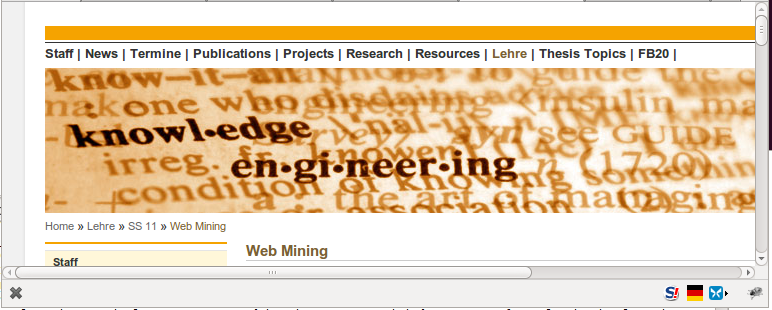
\includegraphics[scale=0.4]{../task05/ke_homepage.png} 
  \caption{The plugin detects german as language for the WebMining Website}
  \label{f:keHomepage}
\end{center}
\end{figure}
	
	
\end{frame}

\begin{frame}[c]
	\myframetitle{Firefox Plugin for language detection}{English}
	%\usepackage{graphics} is needed for \includegraphics
\begin{figure}[htp]
\begin{center}
  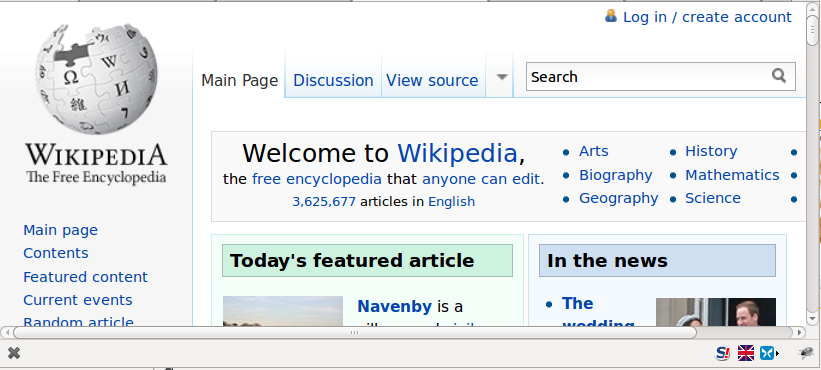
\includegraphics[scale=0.4]{../task05/wikipedia_homepage.png} 
  \caption{The language of en.wikipedia.org is correctly recognized as english}
  \label{f:wpHomepage}
\end{center}
\end{figure}
	
\end{frame}

\begin{frame}[c]
	\myframetitle{Firefox Plugin for language detection}{Norwegian}
	%\usepackage{graphics} is needed for \includegraphics
\begin{figure}[htp]
\begin{center}
  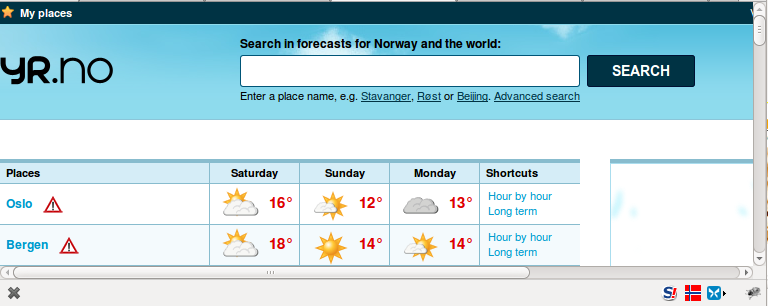
\includegraphics[scale=0.4]{../task05/yr_homepage.png} 
  \caption{The plugin detects norwegian as the language of the weather
  site yr.no}
  \label{figureLabel}
\end{center}
\end{figure}
	
\end{frame}

\begin{frame}[c]
	\myframetitle{Firefox Plugin for language detection}{Failure if p-Tag is
	missing}
	%\usepackage{graphics} is needed for \includegraphics
\begin{figure}[htp]
\begin{center}
  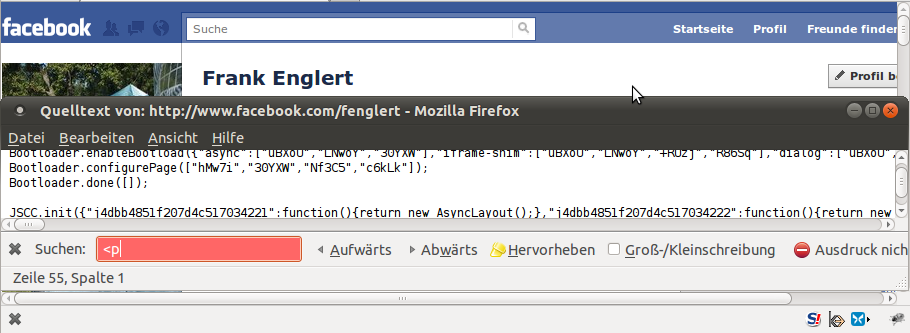
\includegraphics[scale=0.35]{../task05/facebook_homepage.png} 
  \caption{The detection fails if there are no p-Tags indicated by the KE logo}
  \label{figureLabel}
\end{center}
\end{figure}
	
\end{frame}



\begin{frame}[c]
	\myframetitle{Firefox Plugin for language detection}{How it works}
	
	\begin{itemize}
	\fatitem{Implementation details}
	
	\begin{itemize}
		\item Split the text between the '<p>' and '</p>' tags
		\item Count the occurrence of the stop words for german, english and norwegian
		\item Display the icon for the language with the most stop words
	\end{itemize}
		\item ca. 15 LoC without stop word dictionaries
		\fatitem{ good results for such a simple heuristic }
\end{itemize}
\end{frame}

\begin{frame}[c]
\myframetitle{Firefox Plugin for language detection}{Surf session results}
	\begin{table}
		\begin{tabular}{|l|l|l|l|l|}
		\hline 
		URL & \multicolumn{3}{|c|}{Number of stop words} & Correct? \\
		\hline 
		 & de & en & no & \\
		 \hline 
		heise.de & 308 & 18 & 29 & yes\\
		faz.de & 232 & 20 & 21 & yes\\
		ke.tud/.../webmining & 106 & 10 & 14 & yes\\
		gnome.org & 1 & 23 & 1 & yes\\
		kernel.org & 18 & 635 & 37 & yes\\
		yr.no & 10 & 43 & 36 & yes\\
		dagbladet.no & 105 & 548 & 921 & yes\\
		facebook.com/fenglert & 0 & 0 & 0 & no\\
		se.wikipedia.org & 2 & 1 & 0 & -- \\
		fr.wikipedia.org & 22 & 44 & 2 & -- \\
		ja.wikipedia.org & 0 & 0 & 0 & -- \\
		\hline 
		\end{tabular}
		\caption{Language detection Results for a short surf session}
		\label{tblFFPluginResults}
	\end{table}
\end{frame}

\begin{frame}[c]
	\myframetitle{Firefox Plugin for language detection}{Test results}
	\begin{itemize}
	  \fatitem{The results are quite good!}
      \fatitem{ Language correctly detected}
      \begin{itemize}
      	\item on 7 of 8 pages
	  \end{itemize}
      
      \fatitem{But:}
      \begin{itemize}
      	\item Some pages contains multiple languages. e.g yr.no
      	\item The detection fails if a page contains no p-Tags
      	\item The detection yields bogus results if there are no rules for a
      language
	  \end{itemize}
    \end{itemize}
\end{frame}


\end{document}
